\documentclass[12pt,a4paper]{extarticle}
% Copyright 2017 Sergei Tikhomirov, MIT License
% https://github.com/s-tikhomirov/solidity-latex-highlighting/

\usepackage{listings, xcolor}

\definecolor{verylightgray}{rgb}{.97,.97,.97}

\lstdefinelanguage{Solidity}{
	keywords=[1]{anonymous, assembly, assert, balance, break, call, callcode, case, catch, class, constant, continue, constructor, contract, debugger, default, delegatecall, delete, do, else, emit, event, experimental, export, external, false, finally, for, function, gas, if, implements, import, in, indexed, instanceof, interface, internal, is, length, library, log0, log1, log2, log3, log4, memory, modifier, new, payable, pragma, private, protected, public, pure, push, require, return, returns, revert, selfdestruct, send, solidity, storage, struct, suicide, super, switch, then, this, throw, transfer, true, try, typeof, using, value, view, while, with, addmod, ecrecover, keccak256, mulmod, ripemd160, sha256, sha3}, % generic keywords including crypto operations
	keywordstyle=[1]\color{blue}\bfseries,
	keywords=[2]{address, bool, byte, bytes, bytes1, bytes2, bytes3, bytes4, bytes5, bytes6, bytes7, bytes8, bytes9, bytes10, bytes11, bytes12, bytes13, bytes14, bytes15, bytes16, bytes17, bytes18, bytes19, bytes20, bytes21, bytes22, bytes23, bytes24, bytes25, bytes26, bytes27, bytes28, bytes29, bytes30, bytes31, bytes32, enum, int, int8, int16, int24, int32, int40, int48, int56, int64, int72, int80, int88, int96, int104, int112, int120, int128, int136, int144, int152, int160, int168, int176, int184, int192, int200, int208, int216, int224, int232, int240, int248, int256, mapping, string, uint, uint8, uint16, uint24, uint32, uint40, uint48, uint56, uint64, uint72, uint80, uint88, uint96, uint104, uint112, uint120, uint128, uint136, uint144, uint152, uint160, uint168, uint176, uint184, uint192, uint200, uint208, uint216, uint224, uint232, uint240, uint248, uint256, var, void, ether, finney, szabo, wei, days, hours, minutes, seconds, weeks, years},	% types; money and time units
	keywordstyle=[2]\color{teal}\bfseries,
	keywords=[3]{block, blockhash, coinbase, difficulty, gaslimit, number, timestamp, msg, data, gas, sender, sig, value, now, tx, gasprice, origin},	% environment variables
	keywordstyle=[3]\color{violet}\bfseries,
	identifierstyle=\color{black},
	sensitive=false,
	comment=[l]{//},
	morecomment=[s]{/*}{*/},
	commentstyle=\color{gray}\ttfamily,
	stringstyle=\color{red}\ttfamily,
	morestring=[b]',
	morestring=[b]"
}

\lstset{
	language=Solidity,
	backgroundcolor=\color{verylightgray},
	extendedchars=true,
	basicstyle=\footnotesize\ttfamily,
	showstringspaces=false,
	showspaces=false,
	numbers=left,
	numberstyle=\footnotesize,
	numbersep=9pt,
	tabsize=2,
	breaklines=true,
	showtabs=false,
	captionpos=b
}

\usepackage[UTF8]{ctex}
\usepackage{float}
\usepackage{csquotes}
\usepackage{amsmath}
\usepackage{listing}
\usepackage{hyperref}
\usepackage{graphicx}
\usepackage[most]{tcolorbox}
\definecolor{block-gray}{gray}{0.85}
\hypersetup{urlbordercolor={white}, linkbordercolor={white}, citebordercolor={white}}
\graphicspath{ {../images/} }
\newtcolorbox{blockqt}{colback=block-gray,boxrule=0pt,boxsep=0pt,breakable}
\title{ \begin{huge}
\textbf{Epress World: 点对点的世界社区} 
\end{huge} }
\author{ Garbin Huang \\ garbinh@gmail.com \\ epress.world }
\begin{document}
\maketitle
\begin{abstract}
    一种完全点对点的信息交换网络应该允许人们方便地将信息从一个节点发送到另一个节点而不通过中心化服务器。不再将个人隐私和数据存放于第三方中心化服务器,摆脱对大型服务提供商如Facebook、Twitter等的依赖,脱离对大型服务商的依赖意味着人们可以取回个人数据的控制权从而避免隐私侵犯以及潜在的大规模数据泄露带来的威胁。但这只能解决一部分问题,虚假误导性信息泛滥和数字内容盗用问题依然难以避免。我们将提出一种点对点的信息交换网络,同时解决虚假误导信息泛滥和数字内容盗用问题。信息如果要在该网络内流通需要携带不可撤销的信息来源证明,信息接收节点可以方便地对信息来源证明进行验证,只有信息来源被信任并且来源证明有效,信息才会被接收,接收节点会保存完整信息副本,这将帮助减少系统内的虚假误导信息。为了解决数字内容盗用问题,我们还将基于以太坊区块链和智能合约实现信息确权。
\end{abstract}
\section{序言}\label{introduction}
    当今人们的数字生活离不开互联网,离不可数字媒体和社交网络,对它们的依赖带来便利的同时也带来了新的挑战。为了使用这些数字媒体和社交网络提供的服务,人们不得不让渡自己的个人数据使用权给服务提供商\cite{twitter_tos}\cite{facebook_tos},隐私侵犯不可避免。同时由于中心化网络的集中式数据存储,一旦遭受恶意攻击,大规模数据泄露还将带来不可预知的危害。另外,中心化系统缺少有效应对虚假误导信息的机制\cite{twitter_fakenews}\cite{fb_fakenews},恶意攻击者可以以多重匿名身份在系统内散布虚假误导信息不被发现或惩罚从而导致虚假误导信息泛滥。在社区治理上,中心化系统拥有者拥有绝对的控制权,可以删除、屏蔽信息或者直接禁用账号,但这种权力并不一定会被正确使用,由于不同的利益诉求、意识形态和政治倾向不可避免,真正的公平公正事实上是无法做到的。对于数字内容盗用,传统的著作权认定机构难以在无国界的数字世界发挥作用,一方面创作者对于数字内容盗用无能为力,另一方面也将打击创作者的创作积极性。我们无法依赖中心化服务商建立一个自由开放的世界社区。

    我们需要一个不依赖第三方中心化服务器的点对点信息交换网络,该网络允许人们直接完成信息交流而不经过中心化系统。除此之外,网络内流通的信息可被溯源,可被溯源的信息一方面可以帮助信息接收者判断信息源的可靠性,另一方面信息及其来源证明不可撤销也将在一定程度上让人们在发送信息前更加谨慎,在两方面的共同作用下将有望减少虚假误导信息对网络的侵害。我们还需在不依赖传统信用机构的情况下实现信息确权,信息确权除了可以帮助人们解决数字内容盗用问题,由于内容创作者的权益可以得到有效保护,还可能间接促进人们在社区里的高质量内容创作。虚假误导信息被抑制或减少,优秀有价值的信息被鼓励和增加将使社区里的每个人都受益。
    
    事实上,早在Epress World之前,已经有无数组织和个人在这些方面进行过积极探索。比如为了取回个人对个人数据的控制权,欧盟出台的GDPR
    \cite{gdpr}。再比如历史悠久的Diaspora\cite{diaspora},风靡一时的Mastodon\cite{mastodon},以及曾经以太坊联合创始人之一的Mihai Alisie创办的Akasha.World\cite{akasha},他们都是非常优秀的项目,并且都取得了令人瞩目的成就。比特币\cite{bitcoin}的成功实践和以太坊\cite{ethereum}提供的基础设施让我们看到了更好地实现这一切的可能,和比特币\cite{bitcoin}网络不同的是,比特币网络中流通的是一串串代表价值的数字,而在Epress World网络中流通的是人们创造的丰富多彩的信息,比如文字、音频、图像、视频、甚至是任意二进制文件。比特币被定义为世界银行,以太坊被誉为世界计算机,Epress World的愿景是成为更理想的世界社区。

    在本白皮书中,我们将提出一种点对点的信息交换网络,使用不可撤销的信息来源证明(Proof of Source)来实现网络内流通的信息溯源,基于以太坊智能合约实现信息确权。网络中的节点即为社区成员个体,节点之间通过信任关系建立连接,信息只可在相互建立信任连接的节点间传递,节点自行维护信息存储及节点安全。节点的安全是整个网络安全的基石,只要我们确保节点无论被部署在何种网络环境内都可以安全运行,整个网络就是安全的。
\section{总览}
    \begin{figure}[H]
        \centering
        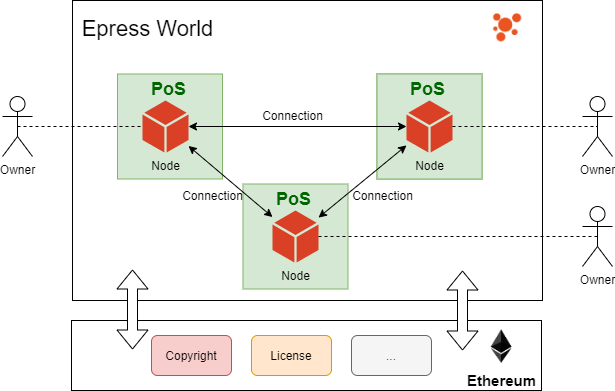
\includegraphics[width=\textwidth]{figures-overview.png}
        \caption{Overview}
    \end{figure}
    如图所示,Epress World主要由点对点的信息交换网络和以太坊智能合约两部分组成,点对点的信息交换网络是Epress World社区的主体,节点是网络的信息生产源,节点通过信任相互连接,信息在Proof of Source(PoS)共识下被允许在网络内传播。以太坊智能合约为Epress World社区赋予信息确权能力。由于我们希望人们的信息交流需求最终都可以摆脱对中心化服务的依赖,社区内流通的信息将被设计为可流通任意形式的数据,并不局限于文字,图片、音频、视频、甚至是任意的二进制文件都将可在社区里流通。
\section{点对点信息交换网络的实现}
    Epress World网络中的节点对应社区中的成员,节点将独自负责数据存储及安全防护。节点间基于信任建立连接,在相互信任的节点间可实现信息传递。为了实现信息溯源,我们提出了信息来源证明(PoS),信息在流通过程中需要确保附带有效的来源证明。节点安全是整个系统安全的基础,Epress World的愿景是成为理想的世界社区,我们希望更多的人可以参与,而不仅仅是面向计算机专家,不限年龄、不限职业、任何人都应该可以轻松且安全地使用。因此,我们需要让节点无论在任何运行环境和任何技术水平管理人员的情况下依然可以安全稳定运行,才能确保系统安全。
\subsection{连接与信任}
    节点之间建立连接在Epress World网络里意味着信任,连接可以是单向的,也可以是双向的。当一个节点创建了一条到另一个节点的连接时,相当于该节点信任来自另一个节点的访问。当两个节点互相添加了到彼此的连接时,双向连接得以建立,这表明该两节点之间彼此信任,彼此接受来自对方的访问以及信息更新。以太坊以及ECDSA非对称加密算法为我们提供了建立这种信任的基石。

    \begin{figure}[H]
        \centering
        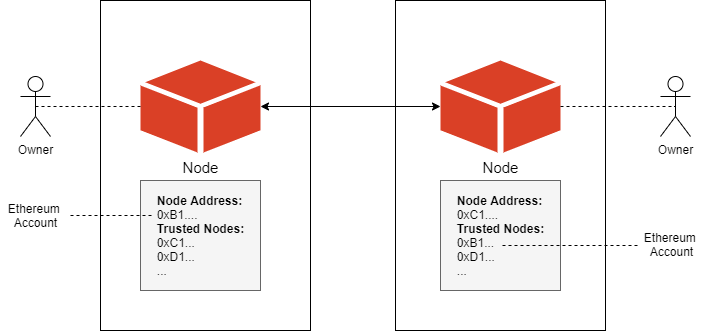
\includegraphics[width=\textwidth]{figures-connect.png}
        \caption{Connect}
    \end{figure}

    如图所示,我们可以将以太坊账户地址做为节点在Epress World网络里的身份标识,与其他节点建立连接相当于在其节点数据库中添加对方节点的以太坊地址为可信地址。
    ~\newline
    \begin{blockqt}
    \textbf{比如:}Alice决定与Bob建立连接,于是他在自己的节点上添加了到Bob节
    点的连接,此时意味着Alice信任Bob,Bob可以访问Alice的节点,获取Alice
    所发布的所有公开信息,当Bob在其节点上添加了到Alice的连接,此时Bob
    和Alice完成了节点间的双向连接。Bob和Alice将可分别通过各自的节点获取对方发布的最新更新,就像在Twitter上获取Following的最新Tweet,或者Facebook上Friend的最新Feed一样。
    \end{blockqt}

    连接可以自由建立,同时也可以自由断开,断开连接相当于节点之间失去信任,主动断开的一方将拒绝来自被断开一方的所有访问请求及信息更新。
\subsection{信息传递与PoS共识}\label{msg_and_pos}
    只有节点间建立了双向连接(也即双向信任关系)后,信息才得以在节点间传递。同时,信息传递过程中需要遵循PoS共识,信息发送节点在发送信息的时候需要同时附带来源证明,信息接收节点收到信息需要验证来源证明,只有当来源证明被验证有效时才接收信息,否则将信息视为不可靠信息丢弃。如图

    \begin{figure}[H]
        \centering
        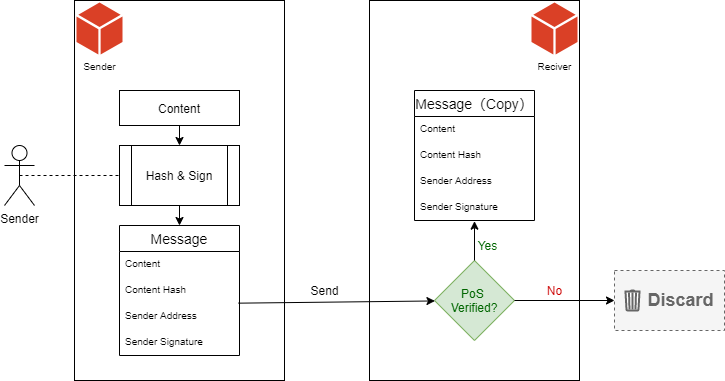
\includegraphics[width=\textwidth]{figures-pos.png}
        \caption{Send Message \& Proof of Source}
    \end{figure}

    由于在发送信息之前,我们已经基于以太坊账户体系建立了节点间的信任关系,节点间彼此存储了对方的以太坊地址,验证PoS共识的过程变得非常简单。首先,信息发送节点通过Hash摘要算法(SHA3)获取待发送信息的摘要信息,信息发送者通过以太坊账户对该摘要信息签发签名,随即将以太坊地址,待发送信息原文,信息摘要以及以太坊签名打包发送给信息接收节点。信息接收节点收到信息后即可非常简单地验证该信息的来源证明,来源证明验证失败,信息接收节点即可将此信息视为不可靠信息直接丢弃。
    ~\newline
    \begin{blockqt}
    \textbf{比如:}Alice(0xB18B7F54eCaD50f22f887702cA2Cd385C5a5332B)与Bob(0x50cBF0471AF07Fd2B4Ee30A5BcE2814Ab2cDe4E0)已建立了双向连接,Alice发布了一条新的文字更新,内容为
    
    \begin{lstlisting}[caption=Message from Alice, numbers=none]
Hello! Bob.
    \end{lstlisting}
    通过SHA3获取到的摘要信息为
    \begin{lstlisting}[caption=SHA3 digest of message, numbers=none, breaklines=true]
0x95251fb76809989bd336326b47954b67a02143e913ce0213bfa26
262dc62f4c3
    \end{lstlisting}
    Alice使用其以太坊账号为该摘要签名
    \begin{lstlisting}[caption=Signature, numbers=none]
0x70b8057ad8984afc1ddf03b521ed45d56a8ee667eff2be7897f45b
a2475f3d655101623b28a1cb8287dac5ec9b5fc1b73697c0304753ad
13f3576e6b3a146b981b
    \end{lstlisting}
    Alice节点将该组信息打包发送给Bob节点,Bob节点收到信息后验证内容与SHA3摘要是否匹配,以防信息在传递过程中被篡改,紧接着验证对该摘要的签名是否来源于Alice的以太坊地址,验证通过则来源证明有效,Bob节点接收该信息并且保存完整副本,Alice和Bob完成了一次典型的信息传递。
    \end{blockqt}
\subsection{Group节点}\label{group_node}
    传统的互联网社区并没有严格要求只有互相建立信任关系的人们之间才可交换信息,恰恰相反,互联网诞生之初就是为了鼓励信息分享而生。比如在Twitter上,任何人都可以创建账号,任何人都可以关注自己感兴趣的账号,一旦关注成功,被关注者可以同时向世界各地的数以亿计的人广播信息。虽然这种开放的信息传播方式一定程度上加剧了虚假误导信息的传播,但也有它积极的一面------扩大了人们的信息源,除了信任的人,还可以从无数陌生人获取信息。

    事实上,人们的信息源不可能仅依赖于已建立信任连接的节点,与陌生人交流,从陌生节点获取重要信息也是人们当前数字生活很重要的一部分。Group节点将成为人们与陌生人之间实现信息交流的桥梁。虽然我们无法与陌生节点直接建立双向连接,但我们可以通过彼此信任的中间人节点建立间接连接,我们将这类中间人节点定义为Group节点。如图所示

    \begin{figure}[H]
        \centering
        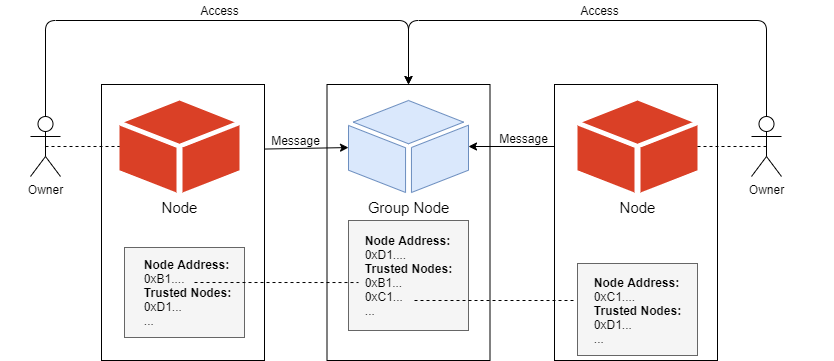
\includegraphics[width=\textwidth]{figures-group.png}
        \caption{Group}
    \end{figure}
    
    Group节点与双方都建立了直接的双向连接,因此,任意一方均可直接对Group节点发送信息更新,又因为节点将保存完整的信息副本,关系中的另一方将可通过访问Group节点获取对方发布的更新信息。从而实现陌生节点间的信息交流。
    \newline
    \begin{blockqt}
    \textbf{比如:}Alice与Carol彼此是陌生人,他们彼此都是比特币爱好者,在Alice
    与Carol认识并建立双向连接前他们无法实现信息交流。很幸运的Isaac是一个热心的比特币爱好者,他在Epress World里建立了一个名叫Bitcoin Group
    的Group节点,任何人都可以自助完成到Bitcoin Group节点的双向连接。Alice和Carol都建立了到Bitcoin Group的双向连接,因此他们都可以向Bitcoin Group发送所有他们想与其他比特币爱好者分享的信息。Carol写了一篇非常棒的比特币协议改进文章,并将该文章签名发送到了Bitcoin Group节点,Alice通过访问Bitcoin Group节点看到了Carol署名的这篇文章,Alice通过Bitcoin Group渠道认识了Carol这个陌生人,并且从这里获取到了这个陌生人撰写的非常棒的关于比特币改进协议的文章。
    \end{blockqt}
\subsection{系统安全}
    节点安全是整个Epress World网络系统安全的基础,我们需要确保任何人可以在尽可能多的环境下安全稳定地运行他们各自的节点,Epress World的节点将被设计为可用于专业机房、小型家庭服务器或NAS、个人PC台式机、笔记本电脑,甚至手机上。因此,我们需要让节点即便是运行在如家庭网络这样没有专业网络防护条件及管理人员的条件下依然安全。我们将从数据安全和节点实例安全两个角度说明我们可以如何实现这一目标。
\subsubsection{数据安全}
    在没有专业网络防护和管理人员的条件下,我们应该假定任意节点被恶意攻击者入侵的概率为100\%。我们需要确保节点被入侵后,敏感数据不被泄露,攻击者无法冒用被入侵节点身份发送信息。

    得益于以太坊的分布式账户设计,我们可以使用以太坊账户做为节点的身份标识,通过签名实现身份认证,因此节点无需存储诸如密码、私钥之类的身份认证信息。这样即便攻击者入侵并获取了节点所在服务器的完整控制权限,由于他并不能获取节点以太坊账户私钥,无法提供有效的数字签名,又由于网络内信息传递受PoS共识约束,所以他无法冒用被入侵节点的身份发送任何信息。

    \begin{figure}[H]
        \centering
        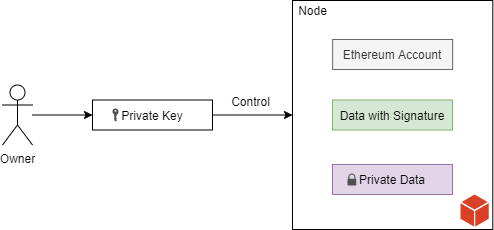
\includegraphics[scale=0.6]{figures-data_security.png}
        \caption{Data Security}
    \end{figure}

    在Epress World的网络里,附带来源证明的信息将被所有接收节点保存完整副本且不可撤销,因此我们将定义附带来源证明的信息为公开信息,由于些信息不可撤销且迟早可能被公之于众,在被攻击者入侵后泄露可能带来的危害有限。但人们同样有存储私密信息的需求,对于私密信息,我们可以使用诸如AES256之类的对称加密算法对内容加密,口令离线保存。这样即便攻击者入侵,也无法获取明文的私密信息。
    ~\newline
    \begin{blockqt}
    \textbf{比如:}Alice的节点被恶意攻击者Mallory入侵,Mallory入侵后想冒用Alice的名义给Alice的所有朋友发送不实的文字更新,他希望Alice的朋友给
    Mallroy的比特币地址转账,Mallory获取了Alice节点所在服务器及数据库的完全访问权限,他在节点的数据库中添加了希望获得比特币转账的不实信息,由于节点间信息传递的PoS共识,该文字信息需要获得节点对应以太坊账号匹配的签名才可被其他节点接收,又由于Alice的以太坊钱包并不存储在节点服务器上,因此Mallory无法获得该文字信息相匹配的数字签名,即便他可以成功将此信息写入Alice的节点数据库,他也无法让Alice的朋友们收到此文字更新,因为没有附带有效来源证明的信息无法在Epress World网络内传播。同时又由于Alice很谨慎地对所有私密数据都进行了加密,Mallory
    也无法查看Alice保存在节点内的所有私密信息。
    \end{blockqt}
\subsubsection{实例安全}
    节点实例运行在没有专业网络防火墙的网络环境下,极易被攻击者通过
    DDoS之类的手段攻击至瘫痪,将影响节点正常参与Epress World社区的权力。而如果人们将节点运行在缺乏有效保护的网络环境下,恶意攻击者将很容易迫使人们无法使用节点。我们需要确保人们面临这种威胁的时候可以有有效的应对措施。

    \begin{figure}[H]
        \centering
        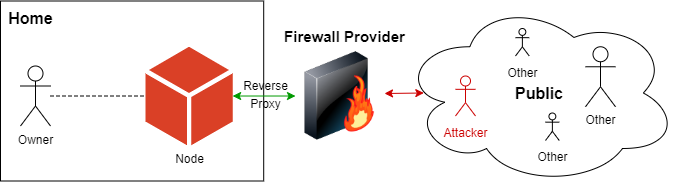
\includegraphics[width=\textwidth]{figures-firewall.png}
        \caption{Firewall}
    \end{figure}

    如图所示,我们假定节点被部署在缺乏有效防护的家庭网络下,为了保障这些节点的安全,我们可以在拥有专业防护条件的机房通过反向代理为这些节点提供安全可靠的网络出口服务。诸如Amazon CloudFront和Clo-
    udflare所提供的服务那样,事实上这已是一个非常成熟的技术和产业。
\section{以太坊区块链及信息确权}
    在传统的互联网社区里缺少独立公正的信用机构为人们的数字内容提供所有权确权服务,导致人们难以主张其对原创内容的所有权,面对信息盗用,内容所有者除了到各大平台举报之外无能为力。如果你的内容在现实中被版权组织认定,或许你可以顺利让盗用者受到惩罚,对于全球化的世界社区,这样的维权成本是高昂的,对于人们的日常创作并不友好。

    以太坊区块链的不可篡改特性及开放的智能合约可以很好地帮助我们实现信息确权。通过智能合约,我们可以将信息以及来源证明(数字签名)做为所有者的所有权证明写入公共的以太坊区块链数据库中,这样即实现了信息确权。


    \begin{figure}[H]
        \centering
        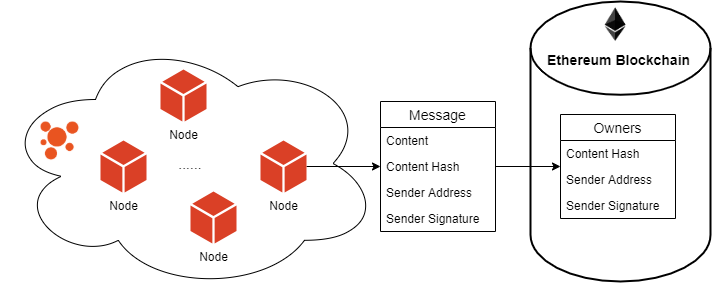
\includegraphics[width=\textwidth]{figures-blockchain.png}
        \caption{Ethereum Blockchain}
    \end{figure}
    
    在章节\ref{msg_and_pos}中我们提到了信息在Epress World网络中的流通,其中包含防止传递过程中被篡改的Content Hash值(Checksum),当内容发生改变,Content Hash也会随之改变,不同的信息总是拥有不同的Content Hash,就像数据的指纹一样。在以太坊区块链中存储完整信息内容是昂贵且不现实的,因此我们可以将该值做为内容等价物写入区块链数据库。
    如图所示,Epress World中的节点将产生的信息及对应的Hash和原创者的以太坊地址以及内容对应的签名发送到Epress World合约,合约校验该Hash是否已被记录(是否已被他人抢先登记所有权),然后合约校验Hash对应的签名与交易发送者是否匹配,校验通过,完成信息确权登记。这样人们就可以通过以太坊区块链中的信息来证明自己是该内容的拥有者。
    ~\newline
    \begin{blockqt}
    \textbf{比如:}Alice与Charlie都是Epress World的社区成员,此前彼此并不相识。Alice发表一篇比特币改进协议的论文,Alice并不想采用开放授权的协议自由共享,因此他第一时间将其登记到以太坊区块链上完成了确权,随后Alice将这篇论文推送到了Bitcoin Group的Group节点与众多比特币爱好者探讨。Charlie通过Bitcoin Group发现了这篇非常棒的论文,随后他将原文复制,没有署名来源于Alice的同时还以自己的名义发布在了他个人的Github账户上。他因为这篇非常棒的论文在Github上获得了不少影响力。一个月后,Alice在Github上发现了自己的这篇论文。随后与Charlie和Github展开交涉。Charlie并不愿承认他盗用了Alice的论文,Github需要证据来判定Charlie是否确实盗用了Alice的论文以做进一步处理。此时,Alice展示了他第一时间在以太坊区块链上登记的确权信息,打包该交易的区块包含时间戳信息,该信息不可篡改,不可伪造。通过比对发现Alice的确权交易所在区块的时间戳信息确实早于Github上Charlie的发布时间。此时Github即可判定Charlie确实盗用了Alice的论文,在明确的证据下,Github对Charlie的盗用行为进行了处理。Alice因为此前第一时间进行了信息确权交易,让本次交涉得以成功。
    \end{blockqt}
\section{社区治理}
    传统的中心化社区服务提供商通常属于个人或者商业公司,他们拥有社区从软件到用户数据一切资源的掌控权。理论上他们可以在任意时间在用户不知情的情况下,查阅、修改、删除、屏蔽任意用户的数据,也可以在任意时间对任意用户账户临时或永久性禁用,这是人们使用其服务的条件,比如Twitter\cite{twitter_tos}和Facebook\cite{facebook_tos}的用户服务条款。在此基础上,他们通常会制定社区规则,当人们触犯规则时将受到惩罚,比如消息被屏蔽或者账户被禁用。这种治理方式在小型的中心化社区通常是高效且不具争议的,但对于全球化的世界社区而言,这种社区治理方式存在明显弊端。首先在规则制定方面,社区拥有者通常会出于其自身利益或国籍所在国利益有一定意识形态和政治倾向。另一方面,在规则执行方面,对于人们是否违规无论是使用机器判定还是人工判定,都会存在一定的误判率,完全的公平公正事实上是做不到的,因此总会有人因误判而受到不应有的处罚。

    我们认为真正的世界社区应该是自由且开放的。任何人可以在任何时候加入或离开社区且不应该存在任何人拥有允许或者禁止他人是否拥有社区参与资格的权力。不应该存在人为制定的社区行为规则以约束人们的信息创作,人们的影响力应该取决于其日积月累的言行,信息的传播应该取决于信息本身而不应该受到社区规则的人为干扰。
    
    \begin{figure}[H]
        \centering
        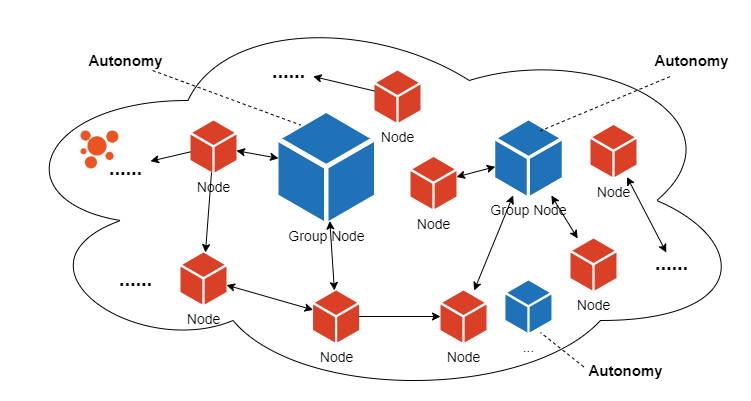
\includegraphics[width=\textwidth]{figures-governance.png}
        \caption{Community Governance Landscape}
    \end{figure}

    如图所示是Epress World的社区治理全景。去中心化的系统架构设计让自由开放的世界社区得以实现,任何人可以在任何时候加入或者离开社区,并且人们的信息创作不需要受任何社区规则的约束。信息的传播也不会受到任何社区规则的约束和人为干扰,只要信息受到人们的欢迎,它们将被广泛传播,相反,如果信息让人们感到厌恶,可能它们只会存在于信息发布者自己的节点里。
    
    任何人都可以创建Group节点用以实现群组交流。Group节点做为小型中心化社区,对于节点创建者来说可能同时存在熟人和陌生人使用该节点进行交流。为了维持秩序,就像大多数中心化社区那样,创建者将制定社区规则。任何人使用Group节点提供服务的同时,都有遵守该节点社区规则的义务。这种区域自治也是Epress World社区治理的重要组成部分。
\section{结论}
    我们已经提出了一种不依赖中心化服务器建立世界社区的方案。从点对点的信息交换网络开始,我们通过让社区成员自行管理维护节点实例和数据取回对个人数据的所有权,避免了隐私侵犯和大规模数据泄露可能带来的威胁。然后,我们通过以太坊及其签名机制实现了节点与节点间的信任互连,让节点间的信息交换成为可能。紧接着,我们引入PoS共识实现信息溯源以帮助提高社区内信息质量,通过引入Group节点让陌生节点间的交流成为可能。最后,我们通过以太坊区块链及其智能合约实现信息确权帮助人们解决数字内容盗用问题。

    我们希望Epress World最终可以让人们完全摆脱对当前各种中心化社区的依赖,无论肤色、种族、国籍,让所有人都可以免于信息垃圾的侵害,从自由平等高效的信息交流中受益,从而实现一个更加理想的世界社区。
\begin{thebibliography}{9}

\bibitem{twitter_tos} 
Twitter Inc.
\textit{Terms of Service}.
\url{https://twitter.com/en/tos}.

\bibitem{facebook_tos} 
Facebook
\textit{Terms of Service}.
\url{https://www.facebook.com/terms.php}.

\bibitem{twitter_fakenews} 
NBC News.
\textit{Twitter is testing new ways to fight misinformation — including a community-based points system}.
\url{https://nbcnews.to/2Vikbfe}, 2020.

\bibitem{fb_fakenews} 
Wired.
\textit{Facebook Is Changing News Feed (Again) to Stop Fake News}.
\url{https://bit.ly/3ebCPhv}, 2019.

\bibitem{gdpr} 
European Parliament, Council of the European Union.
\textit{General Data Protection Regulation}.
\url{https://gdpr-info.eu/}, 2016.

\bibitem{diaspora} 
Diaspora Foundation
\textit{The online social world where you are in control}.
\url{https://diasporafoundation.org/}.

\bibitem{mastodon} 
Mastodon
\textit{Giving social networking back to you}.
\url{https://joinmastodon.org/}.

\bibitem{akasha} 
Mihai Alisie.
\textit{Akasha World}.
\url{https://akasha.org/blog/2017/11/14/new-horizons}, 2017.

\bibitem{bitcoin} 
Satoshi Nakamoto.
\textit{Bitcoin: A Peer-to-Peer Electronic Cash System}. 
\url{https://bitcoin.org/bitcoin.pdf}, 2008.

\bibitem{ethereum} 
Vitalik Buterin.
\textit{A Next-Generation Smart Contract and Decentralized Application Platform}.
\url{https://github.com/ethereum/wiki/wiki/White-Paper}, 2015.

\end{thebibliography}
\pagenumbering{gobble}
\end{document} 